\section[pbdMPI Eg's]{pbdMPI Examples}

\hidenum
\begin{frame}[noframenumbering]
\frametitle{Contents}
 \tableofcontents[currentsection,hideothersubsections,sectionstyle=show/hide]
\end{frame}
\shownum

\subsection{Monte Carlo Simulation}

\begin{frame}[shrink]
  \begin{block}{Example \countex :  Monte Carlo Simulation}\pause
  Sample $N$ uniform observations $(x_i, y_i)$ in the unit square $[0, 1]\times [0,1]$.  Then
\begin{equation*}
\pi \approx 4\left(\frac{\#\ Inside\ Circle}{\#\ Total}\right) = 4\left(\frac{\text{\color{blue}{\# Blue}}}{\text{\color{blue}{\# Blue}}+\text{\color{red}{\# Red}}}\right)
\label{eqn:pi}
\end{equation*}
  \begin{center}
   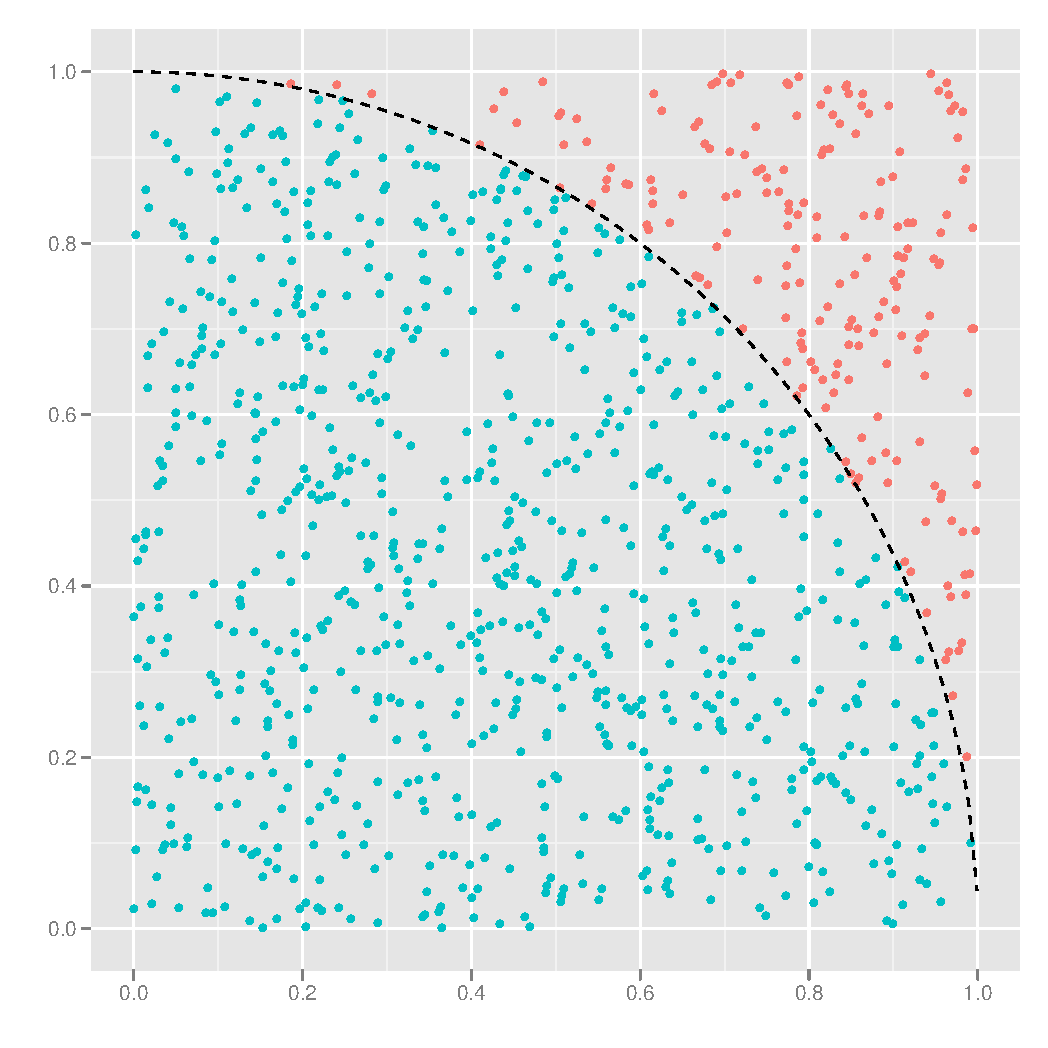
\includegraphics[scale=.25]{pics/pi} 
  \end{center}
  \end{block}
\end{frame}


\begin{frame}[fragile]
  \begin{block}{Example \showex :  Monte Carlo Simulation SPMD Algorithm}\pause
    \begin{enumerate}
     \item Let $n$ be big-ish; we'll take $n=1000$.
     \item Generate an $n\times 2$ matrix $x$ of standard uniform observations.
     \item Count the number of rows satisfying $x^2 + y^2 \leq 1$
     \item Ask everyone else what their answer is; sum it all up.
     \item Take this new answer, multiply by 4 and divide by $n\times nprocs$
     \item If my rank is 0, print the result.
    \end{enumerate}
  \end{block}
\end{frame}


\begin{frame}[fragile,scale,shrink]
  \begin{exampleblock}{Example \showex :  Monte Carlo Simulation Code}\pause
\begin{lstlisting}[title=Serial Code]
N <- 50000
X <- matrix(runif(N * 2), ncol=2)
r <- sum(rowSums(X^2) <= 1)
PI <- 4*r/N
print(PI)
\end{lstlisting}

\begin{lstlisting}[title=Parallel Code]
N.spmd <- 50000 / comm.size()
X.spmd <- matrix(runif(N.spmd * 2), ncol = 2)
r.spmd <- sum(rowSums(X.spmd^2) <= 1)
r <- allreduce(r.spmd)
ret <- allreduce(c(N.spmd, r.spmd), op = "sum")
PI <- 4*r/(N.spmd * comm.size())
comm.print(PI)
\end{lstlisting}

\begin{lstlisting}[title=Sample output]
COMM.RANK = 0
[1] 3.12256
\end{lstlisting}
  \end{exampleblock}
\end{frame}



\subsection{Linear Regression}


\begin{frame}
  \begin{block}{Example \countex :  Linear Regression}\pause
      Find $\bbeta$ such that
      \begin{align*}
      \by = \bX\bbeta + \bepsilon
      \end{align*}

      When $\bX$ is full rank,
      \begin{align*}
      \hat{\bbeta} = (\bX^T\bX)^{-1}\bX^T\by \label{math:ols}
      \end{align*}
  \end{block}
\end{frame}


\begin{frame}
  \begin{block}{Example \showex :  Linear Regression SPMD Algorithm}\pause
    \begin{enumerate}
     \item Compute $tx = x^T$
     \item Compute $A = tx \times x$.  Ask everyone else what they got for this and sum all the answers up.
     \item Compute $B = tx \times yx$.  Ask everyone else what they got for this and sum all the answers up.
     \item Compute $A^{-1}\times B$
    \end{enumerate}
  \end{block}
\end{frame}


\begin{frame}[fragile]
  \begin{exampleblock}{Example \showex :  Linear Regression Code}\pause
\begin{lstlisting}
t.X.spmd <- t(X.spmd)
A <- allreduce(t.X.spmd %*% X.spmd, op = "sum")
B <- allreduce(t.X.spmd %*% y.spmd, op = "sum")

solve(matrix(A, ncol = ncol(X.spmd))) %*% B
\end{lstlisting}
  \end{exampleblock}
\end{frame}

\begin{frame}[fragile]
  \begin{exampleblock}{Example \showex :  Linear Regression Batch Execution}\pause
  Locate the \pkg{pbdDEMO} example script \code{ols.r} and execute:
\vspace{-.4cm}
  \begin{lstlisting}[language=Sh]
### At the shell prompt, run the demo with 4 processors
### Use Rscript.exe for Windows systems
mpirun -np 4 Rscript ols.r
\end{lstlisting}
Sample output:\vspace{-.4cm}
\begin{lstlisting}[language=Sh]
COMM.RANK = 0
          [,1]
[1,] 0.9652591
[2,] 2.0166145
\end{lstlisting}
  \end{exampleblock}
\end{frame}




\subsection{Clustering}


\begin{frame}
  \begin{block}{Example \countex :  Clustering}\pause
      
  \end{block}
\end{frame}